% 41039 Programming 1 revision; shared style copied from the established Week 4 deck.
\documentclass[aspectratio=169]{beamer}
\makeatletter

\usepackage{lmodern}
\usepackage{booktabs}
\usepackage{array}
\usepackage{graphicx}
\usepackage{xcolor}
\usepackage{listings}
\usepackage{pifont}
\usepackage{enumitem}
\usepackage[most]{tcolorbox}
\usepackage{tikz}
\usetikzlibrary{shapes.geometric, arrows.meta, positioning}

% Beamer's default enumerate label expands to itself once enumitem takes the optional
% argument, and TeX runs out of input stack. An explicit label breaks the loop.
\setlist[enumerate]{label=\arabic*.}
\setlist[itemize]{label=\usebeamertemplate{itemize item}}

\definecolor{bkblue}{RGB}{0,70,140}
\definecolor{bktitlebg}{RGB}{64,116,169}
\definecolor{codebg}{RGB}{244,246,249}
\definecolor{codecmt}{RGB}{110,120,130}
\definecolor{codegray}{RGB}{110,120,135}
\definecolor{codestr}{RGB}{150,60,20}
\definecolor{badred}{RGB}{185,40,40}
\definecolor{goodgreen}{RGB}{20,125,70}
\definecolor{srcgrey}{RGB}{105,115,128}

\usetheme{default}
\useinnertheme{rounded}
\setbeamertemplate{navigation symbols}{}

\setbeamercolor{titlelike}{bg=bktitlebg,fg=white}
\setbeamercolor{frametitle}{fg=bkblue,bg=}
\setbeamercolor{author}{fg=bkblue}
\setbeamercolor{institute}{fg=bkblue}
\setbeamercolor{section in toc}{fg=bkblue}
\setbeamerfont{frametitle}{size=\Large,series=\mdseries}
\setbeamerfont{title}{size=\Large,series=\bfseries}
\setbeamerfont{subtitle}{size=\normalsize,series=\bfseries}

\setbeamertemplate{frametitle}{%
  \vspace*{0.35em}%
  \begin{minipage}[b]{0.84\textwidth}%
    \usebeamerfont{frametitle}\usebeamercolor[fg]{frametitle}\insertframetitle%
  \end{minipage}\hfill%
  \begin{minipage}[b]{0.10\textwidth}%
    \raggedleft
\includegraphics[height=0.75cm]{bk-logo.png}%
  \end{minipage}\\[0.1em]%
  {\color{bkblue}\rule{\textwidth}{0.7pt}}%
}

\setbeamercolor{footbar}{bg=bkblue,fg=white}
\setbeamertemplate{footline}{%
  \begin{beamercolorbox}[wd=\paperwidth,ht=2.1ex,dp=1.1ex,leftskip=.3cm,rightskip=.3cm]{footbar}%
    \tiny\insertshorttitle\hfill\insertframenumber{}/\inserttotalframenumber%
  \end{beamercolorbox}%
}

\newcommand{\keyline}[1]{\vfill\begin{center}\textcolor{bkblue}{\textbf{#1}}\end{center}\vspace*{0.2em}}
\newcommand{\hd}[1]{\textbf{#1}}
\newcommand{\code}[1]{\texttt{#1}}
\newcommand{\srcline}[1]{{\color{srcgrey}\scriptsize #1\par}}
\newcommand{\srclink}[2]{\href{#1}{\texttt{#2}}}
\newcommand{\badlabel}[1]{\textcolor{badred}{\ding{55}~\textbf{#1}}}
\newcommand{\goodlabel}[1]{\textcolor{goodgreen}{\ding{51}~\textbf{#1}}}
\newcommand{\neutrallabel}[1]{\textcolor{bkblue}{\textbf{#1}}}
\newcommand{\timing}[2]{\hfill{\small\textcolor{bkblue}{\textbf{#1 \textbullet{} #2}}}}
% a blank to be filled in, numbered so the word bank can be checked against it
\newcommand{\blank}[1]{\underline{\hspace{1.1em}\textbf{(#1)}\hspace{1.1em}}}
\newcommand{\yes}{\textcolor{goodgreen}{\ding{51}}}
\newcommand{\no}{\textcolor{badred}{\ding{55}}}

% --- Stack and heap pictures (Draw it) --------------------------------------
\tikzset{
  sframe/.style={draw=bkblue, thick, fill=codebg, rounded corners=2pt, inner sep=4pt,
    font=\scriptsize\ttfamily, align=left, anchor=north west},
  ftitle/.style={font=\scriptsize\sffamily\bfseries, text=bkblue, anchor=south west},
  cell/.style={draw=bkblue, fill=white, font=\scriptsize\ttfamily, minimum width=0.62cm,
    minimum height=0.5cm, inner sep=1pt},
  atitle/.style={font=\scriptsize\ttfamily, text=bkblue, anchor=south west, inner sep=1pt},
  ref/.style={-{Stealth[length=5pt]}, thick, draw=bkblue!85!black},
  hd/.style={font=\small\sffamily\bfseries, text=bkblue},
}

\hypersetup{colorlinks=true, urlcolor=bkblue, linkcolor=bkblue}

% --- Question box: what the room is being asked --------------------------
\newtcolorbox{discussionbox}[1]{
  title=\textbf{#1}, coltitle=bkblue, colback=white, colframe=bkblue,
  colbacktitle=bkblue!10, boxrule=1pt, arc=3pt,
  left=6pt, right=6pt, top=4pt, bottom=4pt
}
% --- Answer box: revealed after they have committed to an answer ---------
\newtcolorbox{contextbox}[1]{
  title=\textbf{#1}, coltitle=white, colback=bkblue!5, colframe=bkblue,
  colbacktitle=bkblue!80, boxrule=0.6pt, arc=3pt,
  left=6pt, right=6pt, top=4pt, bottom=4pt
}

\lstdefinestyle{code}{
  basicstyle=\ttfamily\scriptsize,
  keywordstyle=\color{bkblue}\bfseries,
  commentstyle=\color{codecmt}\itshape,
  stringstyle=\color{codestr},
  backgroundcolor=\color{codebg},
  frame=leftline, framerule=1.2pt, rulecolor=\color{bkblue},
  xleftmargin=1.1em, framexleftmargin=1.1em,
  framexrightmargin=0.4em, framextopmargin=3pt, framexbottommargin=3pt,
  showstringspaces=false, columns=fullflexible, keepspaces=true,
  breaklines=true, aboveskip=0.6em, belowskip=0.6em,
}
\lstdefinestyle{bad}{style=code, rulecolor=\color{badred}, backgroundcolor=\color{badred!4}}
\lstdefinestyle{good}{style=code, rulecolor=\color{goodgreen}, backgroundcolor=\color{goodgreen!5}}
\lstset{style=code}
% listings' Python predates 3.10; teach it the soft keywords and constants this deck uses
\lstdefinelanguage{Py}[]{Python}{morekeywords={match,case,elif,True,False}}

\setbeamertemplate{title page}{%
  \vspace*{0.5em}
  \begin{centering}
    \begin{beamercolorbox}[sep=8pt,center,rounded=true,shadow=false]{title}
      \usebeamerfont{title}\inserttitle\par
      \ifx\insertsubtitle\@empty\else
        \vskip0.4em{\usebeamerfont{subtitle}\insertsubtitle\par}
      \fi
    \end{beamercolorbox}
    \vskip1.0em
    
\includegraphics[height=1.7cm]{bk-logo.png}
    \vskip1.0em
    {\usebeamercolor[fg]{author}\usebeamerfont{author}\insertauthor\par}
    \vskip0.5em
    {\usebeamercolor[fg]{institute}\usebeamerfont{institute}\insertinstitute\par}
    \vskip0.6em
    {\usebeamerfont{date}\insertdate\par}
  \end{centering}
}




\title[41039 Programming 1 --- Revision of Week 10]{41039 Programming 1}
\subtitle{Revision of Week 10: Writing files and reliable reports}
\author{Dr. Xuan-Bach Le\\ \small\texttt{le.xuan.bach@hcmut.edu.vn}}
\institute{\small Faculty of Computer Science and Engineering, HCMUT}
\date{September Session 2026}
\AtBeginSection[]{\begin{frame}{Outline}\tableofcontents[currentsection]\end{frame}}
\begin{document}

\begin{frame}{}
\titlepage
\end{frame}

\begin{frame}{How the revision session works}
\begin{discussionbox}{A recap before the next lecture}\small Write an answer before the reveal. Explain the state change, rule or contract that makes it follow. These are practice questions, with no new assessment requirements.\end{discussionbox}
\begin{columns}[T,onlytextwidth]
\column{0.48\textwidth}
\raggedright
\neutrallabel{Part 1: on your own}\begin{itemize}\small\item 6 short questions\item About 90 seconds per question\item Java and Python; name the language first\end{itemize}
\column{0.48\textwidth}
\raggedright
\neutrallabel{Part 2: teams of 3 or 4}\begin{itemize}\small\item Draw the model\item Spot the errors\item Predict the output\item Write and test the code\end{itemize}
\end{columns}
\keyline{A result needs a reason. A repair needs a counterexample.}
\end{frame}

\section{On your own}

\begin{frame}[fragile]{1. A writer can target memory}
\srcline{Java 8 excerpt: main statements and supporting types; commit to an outcome before the reveal.}
\begin{columns}[T,onlytextwidth]
\column{0.62\textwidth}
\raggedright
\begin{lstlisting}[style=code,language=Java]
import java.io.*;
StringWriter buffer=new StringWriter();
try(PrintWriter writer=new PrintWriter(buffer)) {
    writer.println("name,mark");
    writer.println("Linh,85");
}
System.out.print(buffer.toString());
\end{lstlisting}

\column{0.34\textwidth}
\raggedright
\begin{onlyenv}<1>\begin{discussionbox}{Your answer}\small What is the complete output? Which line or rule decides it?\end{discussionbox}\end{onlyenv}
\begin{onlyenv}<2>\begin{contextbox}{Answer}
\begin{lstlisting}[style=code]
name,mark
Linh,85
\end{lstlisting}
\scriptsize\raggedright The writer emits the header then the record. The buffer lets the page show exactly what would be written.
\end{contextbox}\end{onlyenv}
\end{columns}

\end{frame}

\begin{frame}[fragile]{2. Python write does not add a newline}
\srcline{Python 3; commit to an outcome before the reveal.}
\begin{columns}[T,onlytextwidth]
\column{0.62\textwidth}
\raggedright
\begin{lstlisting}[style=code,language=Py]
from io import StringIO
buffer=StringIO()
buffer.write("tea")
buffer.write("coffee")
print(repr(buffer.getvalue()))
buffer.close()
\end{lstlisting}

\column{0.34\textwidth}
\raggedright
\begin{onlyenv}<1>\begin{discussionbox}{Your answer}\small What is the complete output? Which line or rule decides it?\end{discussionbox}\end{onlyenv}
\begin{onlyenv}<2>\begin{contextbox}{Answer}
\begin{lstlisting}[style=code]
'teacoffee'
\end{lstlisting}
\scriptsize\raggedright The two writes concatenate; print adds a newline only when displaying the representation.
\end{contextbox}\end{onlyenv}
\end{columns}

\end{frame}

\begin{frame}[fragile]{3. Java file output and read-back on Ed}
\srcline{Java 8 excerpt: main statements and supporting types; commit to an outcome before the reveal.}
\begin{columns}[T,onlytextwidth]
\column{0.62\textwidth}
\raggedright
\begin{lstlisting}[style=code,language=Java]
import java.io.*;
File file=new File("report.txt");
try(PrintWriter out=new PrintWriter(file,"UTF-8")) {
    out.println("name,mark");
    out.println("Linh,85");
    if(out.checkError()) throw new IOException("write failed");
}
try(BufferedReader in=new BufferedReader(new InputStreamReader(new FileInputStream(file),"UTF-8"))) {
    String line;
    while((line=in.readLine())!=null) System.out.println(line);
}
\end{lstlisting}

\column{0.34\textwidth}
\raggedright
\begin{onlyenv}<1>\begin{discussionbox}{Your answer}\small Predict the output. Why close before reading back? Do PrintWriter write failures always throw IOException?\end{discussionbox}\end{onlyenv}
\begin{onlyenv}<2>\begin{contextbox}{Answer}
\begin{lstlisting}[style=code]
name,mark
Linh,85
\end{lstlisting}
\scriptsize\raggedright Closing completes the output before a reader opens the file. Records appear in their written order. PrintWriter stores many write failures instead of throwing them; checkError reports those failures. Closing manages resource lifetime but does not prove that every write succeeded.
\end{contextbox}\end{onlyenv}
\end{columns}

\end{frame}

\begin{frame}[fragile]{4. Use CSV tooling when fields need quoting}
\srcline{Python 3; commit to an outcome before the reveal.}
\begin{columns}[T,onlytextwidth]
\column{0.62\textwidth}
\raggedright
\begin{lstlisting}[style=code,language=Py]
import csv
from io import StringIO
buffer=StringIO(newline="")
writer=csv.writer(buffer,lineterminator="\n")
writer.writerow(["name","mark"])
writer.writerow(["An, Mai",85])
print(buffer.getvalue(),end="")
buffer.seek(0)
rows=list(csv.reader(buffer))
print(rows[1][0])
buffer.close()
\end{lstlisting}

\column{0.34\textwidth}
\raggedright
\begin{onlyenv}<1>\begin{discussionbox}{Your answer}\small What is the complete output? Which line or rule decides it?\end{discussionbox}\end{onlyenv}
\begin{onlyenv}<2>\begin{contextbox}{Answer}
\begin{lstlisting}[style=code]
name,mark
"An, Mai",85
An, Mai
\end{lstlisting}
\scriptsize\raggedright CSV quotes the name containing a comma; the reader returns the original field without the quoting characters.
\end{contextbox}\end{onlyenv}
\end{columns}

\end{frame}

\begin{frame}[fragile]{5. Format records separately from saving them}
\srcline{Java 8; commit to an outcome before the reveal.}
\begin{columns}[T,onlytextwidth]
\column{0.62\textwidth}
\raggedright
\begin{lstlisting}[style=code,language=Java]
public class Demo {
    static String format(String name,int mark) { return name+","+mark; }
    public static void main(String[] args) {
        String[] names={"Linh","An"};
        int[] marks={85,49};
        for(int i=0;i<names.length;i++) System.out.println(format(names[i],marks[i]));
    }
}
\end{lstlisting}

\column{0.34\textwidth}
\raggedright
\begin{onlyenv}<1>\begin{discussionbox}{Your answer}\small What is the complete output? Which line or rule decides it?\end{discussionbox}\end{onlyenv}
\begin{onlyenv}<2>\begin{contextbox}{Answer}
\begin{lstlisting}[style=code]
Linh,85
An,49
\end{lstlisting}
\scriptsize\raggedright The formatter pairs each name with the corresponding mark; persistence is a separate choice.
\end{contextbox}\end{onlyenv}
\end{columns}

\end{frame}

\begin{frame}[fragile]{6. Round-trip a small document}
\srcline{Python 3; commit to an outcome before the reveal.}
\begin{columns}[T,onlytextwidth]
\column{0.62\textwidth}
\raggedright
\begin{lstlisting}[style=code,language=Py]
import json
record={"name":"Linh","marks":[85,90]}
text=json.dumps(record,sort_keys=True)
restored=json.loads(text)
print(restored["name"])
print(sum(restored["marks"]))
print(restored==record)
\end{lstlisting}

\column{0.34\textwidth}
\raggedright
\begin{onlyenv}<1>\begin{discussionbox}{Your answer}\small What is the complete output? Which line or rule decides it?\end{discussionbox}\end{onlyenv}
\begin{onlyenv}<2>\begin{contextbox}{Answer}
\begin{lstlisting}[style=code]
Linh
175
True
\end{lstlisting}
\scriptsize\raggedright The round trip preserves the two marks and name; their sum is 175.
\end{contextbox}\end{onlyenv}
\end{columns}

\end{frame}

\section{Team round 1: draw the model}

\begin{frame}{Form teams}
\begin{itemize}[itemsep=0.8em]\item Teams of 3 or 4. One shared sheet, one spokesperson.\item For each challenge, record the result and the reason.\item Rotate the spokesperson. Other teams can challenge an explanation.\item The final task has starter files and a Java/Python solution pair.\end{itemize}\keyline{Discuss first. Commit to an answer. Then compare with the reveal.}
\end{frame}

\begin{frame}[fragile]{Draw it: One report, several responsibilities}
\begin{columns}[T,onlytextwidth]
\column{0.62\textwidth}
\raggedright
\begin{lstlisting}[style=code,language=Java]
import java.io.*;
int[] marks={85,49,50};
int total=0,passed=0;
for(int mark:marks) { total+=mark; if(mark>=50) passed++; }
StringWriter text=new StringWriter();
try(PrintWriter out=new PrintWriter(text)) {
    out.println("count,total,passed");
    out.println(marks.length+","+total+","+passed);
}
System.out.print(text.toString());
\end{lstlisting}

\column{0.34\textwidth}
\raggedright
\begin{discussionbox}{Four minutes}\small Draw the flow and responsibilities after the shown operations. Label the important state. Mark what is shared, what changes, or which path handles failure. Predict every output line.\end{discussionbox}
\end{columns}
\par\srcline{\href{../../weeks/week-10.html}{Course website: Week 10}. Complete programs accompany this deck.}

\end{frame}

\begin{frame}[fragile]{Draw it: one answer}
\begin{columns}[T,onlytextwidth]
\column{0.66\textwidth}
\raggedright
\resizebox{\linewidth}{!}{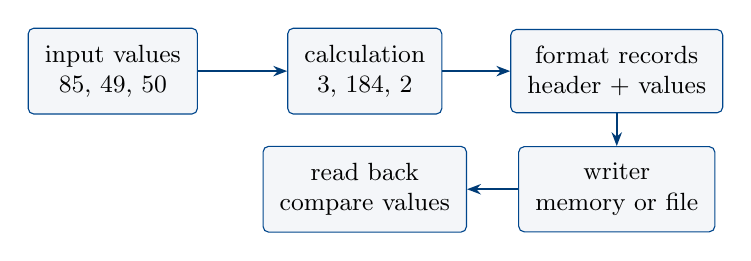
\begin{tikzpicture}
\node[draw=bkblue,rounded corners=2pt,fill=codebg,align=center,inner sep=6pt,font=\small] (read) at (0,0) {input values\\[0pt] 85, 49, 50};
\node[draw=bkblue,rounded corners=2pt,fill=codebg,align=center,inner sep=6pt,font=\small] (calc) at (3.2,0) {calculation\\[0pt] 3, 184, 2};
\node[draw=bkblue,rounded corners=2pt,fill=codebg,align=center,inner sep=6pt,font=\small] (format) at (6.4,0) {format records\\[0pt] header + values};
\node[draw=bkblue,rounded corners=2pt,fill=codebg,align=center,inner sep=6pt,font=\small] (write) at (6.4,-1.5) {writer\\[0pt] memory or file};
\node[draw=bkblue,rounded corners=2pt,fill=codebg,align=center,inner sep=6pt,font=\small] (readback) at (3.2,-1.5) {read back\\[0pt] compare values};
\draw[ref] (read) -- (calc);
\draw[ref] (calc) -- (format);
\draw[ref] (format) -- (write);
\draw[ref] (write) -- (readback);
\end{tikzpicture}}

\column{0.3\textwidth}
\raggedright
\begin{contextbox}{Output}\begin{lstlisting}[style=code]
count,total,passed
3,184,2
\end{lstlisting}
\end{contextbox}
\end{columns}
\vspace{0.8em}
\small Calculation produces values, formatting chooses a representation, and writing chooses a destination. A read-back test must inspect values and delimiters, not only whether an exception occurred.
\par\srcline{\href{../../weeks/week-10.html}{Course website: Week 10}. Complete programs accompany this deck.}

\end{frame}

\section{Team round 2: spot the errors}

\begin{frame}[fragile]{Spot the errors 1: Java (5 min)}
\begin{discussionbox}{Contract}\small Emit exactly three CSV lines: a header, Linh,85 and An,49. Names contain no commas or newlines.\end{discussionbox}
\begin{columns}[T,onlytextwidth]
\column{0.48\textwidth}
\raggedright
\begin{lstlisting}[style=bad,language=Java,numbers=left,numberstyle=\tiny\color{codegray},firstnumber=1,numbersep=0.7em]
import java.io.*;
public class Broken {
    public static void main(String[] args) {
        StringWriter buffer=new StringWriter();
        PrintWriter out=new PrintWriter(buffer);
        String[] names={"Linh","An"};
        int[] marks={85,49};
\end{lstlisting}

\column{0.48\textwidth}
\raggedright
\begin{lstlisting}[style=bad,language=Java,numbers=left,numberstyle=\tiny\color{codegray},firstnumber=8,numbersep=0.7em]
        out.print("name,mark");
        for(int i=0;i<names.length;i++) {
            out.print(names[i]+marks[i]);
        }
        System.out.print(buffer.toString());
    }
}
\end{lstlisting}

\end{columns}

\end{frame}

\begin{frame}[fragile]{Spot the errors 1: answers}
\begin{columns}[T,onlytextwidth]
\column{0.58\textwidth}
\raggedright
\begin{contextbox}{The repairs}\footnotesize\begin{itemize}[itemsep=0.45em]\item \textbf{L8:} Terminate the header with println.\item \textbf{L10:} Insert the field delimiter and terminate every record.\item \textbf{L12:} Close the writer before reading back the stored text. A memory writer may hide missing-flush bugs.\end{itemize}\end{contextbox}
\column{0.38\textwidth}
\raggedright
\badlabel{Original program}\begin{lstlisting}[style=code]
name,markLinh85An49
\end{lstlisting}
\goodlabel{After the repairs}\begin{lstlisting}[style=code]
name,mark
Linh,85
An,49
\end{lstlisting}

\end{columns}
\par\srcline{\href{../../weeks/week-10.html}{Course website: Week 10}. Complete programs accompany this deck.}

\end{frame}

\begin{frame}[fragile]{Spot the errors 2: Python (5 min)}
\begin{discussionbox}{Contract}\small Append a complete new record to the existing old record. The resulting file must contain old and new on separate lines.\end{discussionbox}
\begin{columns}[T,onlytextwidth]
\column{0.48\textwidth}
\raggedright
\begin{lstlisting}[style=bad,language=Py,numbers=left,numberstyle=\tiny\color{codegray},firstnumber=1,numbersep=0.7em]
from pathlib import Path
from tempfile import TemporaryDirectory
with TemporaryDirectory() as folder:
    path=Path(folder)/"report.txt"
    path.write_text("old\n",encoding="utf-8")
\end{lstlisting}

\column{0.48\textwidth}
\raggedright
\begin{lstlisting}[style=bad,language=Py,numbers=left,numberstyle=\tiny\color{codegray},firstnumber=6,numbersep=0.7em]
    with path.open("w",encoding="utf-8") as out:
        out.write("new")
    with path.open("r",encoding="utf-8") as source:
        print(source.read(),end="")
\end{lstlisting}

\end{columns}

\end{frame}

\begin{frame}[fragile]{Spot the errors 2: answers}
\begin{columns}[T,onlytextwidth]
\column{0.58\textwidth}
\raggedright
\begin{contextbox}{The repairs}\footnotesize\begin{itemize}[itemsep=0.45em]\item \textbf{L6:} Use append mode to retain old content.\item \textbf{L7:} Add the record terminator explicitly. write does not add a newline.\end{itemize}\end{contextbox}
\column{0.38\textwidth}
\raggedright
\badlabel{Original program}\begin{lstlisting}[style=code]
new
\end{lstlisting}
\goodlabel{After the repairs}\begin{lstlisting}[style=code]
old
new
\end{lstlisting}

\end{columns}
\par\srcline{\href{../../weeks/week-10.html}{Course website: Week 10}. Complete programs accompany this deck.}

\end{frame}

\section{Team round 3: predict the output}

\begin{frame}[fragile]{Predict 1: A writer preserves exact characters}
\begin{columns}[T,onlytextwidth]
\column{0.62\textwidth}
\raggedright
\begin{lstlisting}[style=code,language=Java]
import java.io.*;
StringWriter buffer=new StringWriter();
try(PrintWriter out=new PrintWriter(buffer)) {
    out.print("A");
    out.println("B");
    out.println("C");
}
System.out.print(buffer.toString());
System.out.println("D");
\end{lstlisting}

\column{0.34\textwidth}
\raggedright
\begin{discussionbox}{Three minutes}\small Write every line in order. Explain the first state change, alias, dispatch decision or exception that controls the result. Then propose one change that alters the output.\end{discussionbox}
\end{columns}
\par\srcline{\href{../../weeks/week-10.html}{Course website: Week 10}. Complete programs accompany this deck.}

\end{frame}

\begin{frame}[fragile]{Predict 1: answer}
\begin{columns}[T,onlytextwidth]
\column{0.42\textwidth}
\raggedright
\begin{lstlisting}[style=code]
AB
C
D
\end{lstlisting}

\column{0.54\textwidth}
\raggedright
\begin{contextbox}{Why}\small print writes no terminator. The first println completes AB; the next completes C. D goes to standard output after the stored text.\end{contextbox}
\end{columns}
\par\srcline{\href{../../weeks/week-10.html}{Course website: Week 10}. Complete programs accompany this deck.}

\end{frame}

\begin{frame}[fragile]{Predict 2: Quoting and a read-back test}
\begin{columns}[T,onlytextwidth]
\column{0.62\textwidth}
\raggedright
\begin{lstlisting}[style=code,language=Py]
import csv
from io import StringIO
text=StringIO(newline="")
writer=csv.writer(text,lineterminator="\n")
writer.writerow(["An, Mai",50])
writer.writerow(["Tea",49])
text.seek(0)
rows=list(csv.reader(text))
print(len(rows))
print(rows[0][0],int(rows[0][1])>=50)
print(rows[1])
\end{lstlisting}

\column{0.34\textwidth}
\raggedright
\begin{discussionbox}{Three minutes}\small Write every line in order. Explain the first state change, alias, dispatch decision or exception that controls the result. Then propose one change that alters the output.\end{discussionbox}
\end{columns}
\par\srcline{\href{../../weeks/week-10.html}{Course website: Week 10}. Complete programs accompany this deck.}

\end{frame}

\begin{frame}[fragile]{Predict 2: answer}
\begin{columns}[T,onlytextwidth]
\column{0.42\textwidth}
\raggedright
\begin{lstlisting}[style=code]
2
An, Mai True
['Tea', '49']
\end{lstlisting}

\column{0.54\textwidth}
\raggedright
\begin{contextbox}{Why}\small The CSV writer quotes the comma in the name. The reader reconstructs one field containing that comma; the mark is converted before comparing it numerically.\end{contextbox}
\end{columns}
\par\srcline{\href{../../weeks/week-10.html}{Course website: Week 10}. Complete programs accompany this deck.}

\end{frame}

\section{Team round 4: write the code}

\begin{frame}[fragile]{Code it: specification}
\begin{discussionbox}{A report with a stable schema}\small Read n then n marks in 0..100. Print count,total,passed and one CSV record with the number of marks, their sum, and the number at least 50. Standard output is the test destination; the same formatter could feed a file writer.\end{discussionbox}
\begin{columns}[T,onlytextwidth]
\column{0.48\textwidth}
\raggedright
\neutrallabel{Example input}\begin{lstlisting}[style=code]
3
85 49 50
\end{lstlisting}

\column{0.48\textwidth}
\raggedright
\neutrallabel{Expected output}\begin{lstlisting}[style=code]
count,total,passed
3,184,2
\end{lstlisting}

\end{columns}
\small Eight minutes. One Java team and one Python team at the keyboard. Other teams produce a boundary test and explain which wrong implementation it would expose.
\end{frame}

\begin{frame}[fragile]{Code it: Java solution}
\begin{lstlisting}[style=code,language=Java,numbers=left,numberstyle=\tiny\color{codegray},firstnumber=1,numbersep=0.7em]
import java.util.Scanner;
Scanner sc=new Scanner(System.in);
int n=sc.nextInt(),total=0,passed=0;
for(int i=0;i<n;i++) { int mark=sc.nextInt(); total+=mark; if(mark>=50) passed++; }
System.out.println("count,total,passed");
System.out.println(n+","+total+","+passed);
\end{lstlisting}
\par\srcline{\href{../../weeks/week-10.html}{Course website: Week 10}. Complete programs accompany this deck.}

\end{frame}

\begin{frame}[fragile]{Code it: Python solution}
\begin{lstlisting}[style=code,language=Py,numbers=left,numberstyle=\tiny\color{codegray},firstnumber=1,numbersep=0.7em]
n=int(input())
marks=list(map(int,input().split()))[:n]
print("count,total,passed")
print(f"{n},{sum(marks)},{sum(mark>=50 for mark in marks)}")
\end{lstlisting}
\par\srcline{\href{../../weeks/week-10.html}{Course website: Week 10}. Complete programs accompany this deck.}

\end{frame}

\begin{frame}{Code it: the tests}
\footnotesize {\scriptsize A slash separates input lines; (blank) denotes an empty line.\par}\medskip \textbf{Test 1}\par \code{3 / 85 49 50}\par \textbf{Output:} \code{count,total,passed / 3,184,2}\par\medskip \textbf{Test 2}\par \code{0 / (blank)}\par \textbf{Output:} \code{count,total,passed / 0,0,0}\par\medskip \textbf{Test 3}\par \code{3 / 0 0 0}\par \textbf{Output:} \code{count,total,passed / 3,0,0}\par\medskip \textbf{Test 4}\par \code{2 / 100 50}\par \textbf{Output:} \code{count,total,passed / 2,150,2}\par\medskip \keyline{Explain why each test is present, not only whether it passes.}
\end{frame}

\section{Wrapping up}

\begin{frame}{What you should now be able to explain}
\begin{itemize}[itemsep=0.6em]\item Specify delimiters, newlines, field order and text encoding.\item Distinguish write, append and read modes.\item Separate computation from formatting and persistence.\item Use quoting for general CSV and inspect values after reading back.\end{itemize}\vfill\small Return to the matching week page for runnable examples and further practice. Bring one unresolved prediction or counterexample to the next class.\par\srcline{\href{../../weeks/week-10.html}{Course website: Week 10}. Complete programs accompany this deck.}

\end{frame}

\end{document}
